\documentclass[10pt]{article}
\usepackage[letterpaper,left=1in,right=1in,top=1in,bottom=1in,portrait]{geometry}

\usepackage{amsmath,amssymb}
\usepackage{bbm}

\usepackage[none]{hyphenat}
\usepackage{parskip}

\usepackage{graphicx}

\usepackage[sc]{mathpazo}
\linespread{1.05}         % Palladio needs more leading (space between lines)
\usepackage[ttdefault=true]{AnonymousPro}
\usepackage[T1]{fontenc}

\usepackage{enumerate}

\usepackage{titlesec}
\titleformat{\section}
  {\itshape\large}
  {\thesection}
  {}
  {}
\titleformat{\subsection}
  {\itshape}
  {\thesubsection}
  {}
  {}

\makeatletter
\renewcommand\@maketitle
{ 
    {\LARGE \emph{\@title} \par }
    {\small \@author \par}
}
\makeatother

\title{nom-inator}
\author
{
    Project 1 \\
    COMS W4111 \\
    Introduction to Databases \\\\
    Chih-Sheng Wang (cw2952)\\
    Hang Su (hs2761)
}
\date

\begin{document}

\maketitle

\section*{Proposal}

The \emph{nom-inator} is a restaurant reccommendation app that will draw on the Foursquare API, weather reports, as well as the user's location and preferences to recommend restaurants for the user to try out.

\subsection*{Databases needed}
\begin{enumerate}
\item{Restaurant information, along with visit information and their timestamps (Foursquare)}
\item{Weather data, past and present}
\end{enumerate}

\subsection*{Use Cases}

\begin{enumerate}
\item
{
    Filter and sort restaurants that fit a user's requirements at a specific moment in time based on
    \begin{enumerate}
    \item{a restaurant's waiting time / popularity;}
    \item{the current time, the day of the week, the weather, and the user's current location; and}
    \item{the user's list of favourite restaurants.}
    \end{enumerate}
}
\item{Recommend the best days and times to visit a user-specified restaurant.}
\item{Users can maintain a list of favourite restaurants, that feed into the results for use case 1.}
\end{enumerate}

\subsection*{Potential Problems}
\begin{enumerate}
\item{Need information about restaurants' opening hours to avoid erroneous recommendations.}
\item{How do we efficiently find restaurants near to the user?}
\end{enumerate}

\subsection*{Other Applications}
The same recommmendation system can potentially be applied to other popular places like museums and tourist attractions.

\subsection*{Contingency Plan}
Eliminate use cases 3 and 1c (i.e. the favourites list will not be implemented), as well as use case 1b (i.e. the geolocation search will not be implemented).

\pagebreak

\section*{ER Diagram}

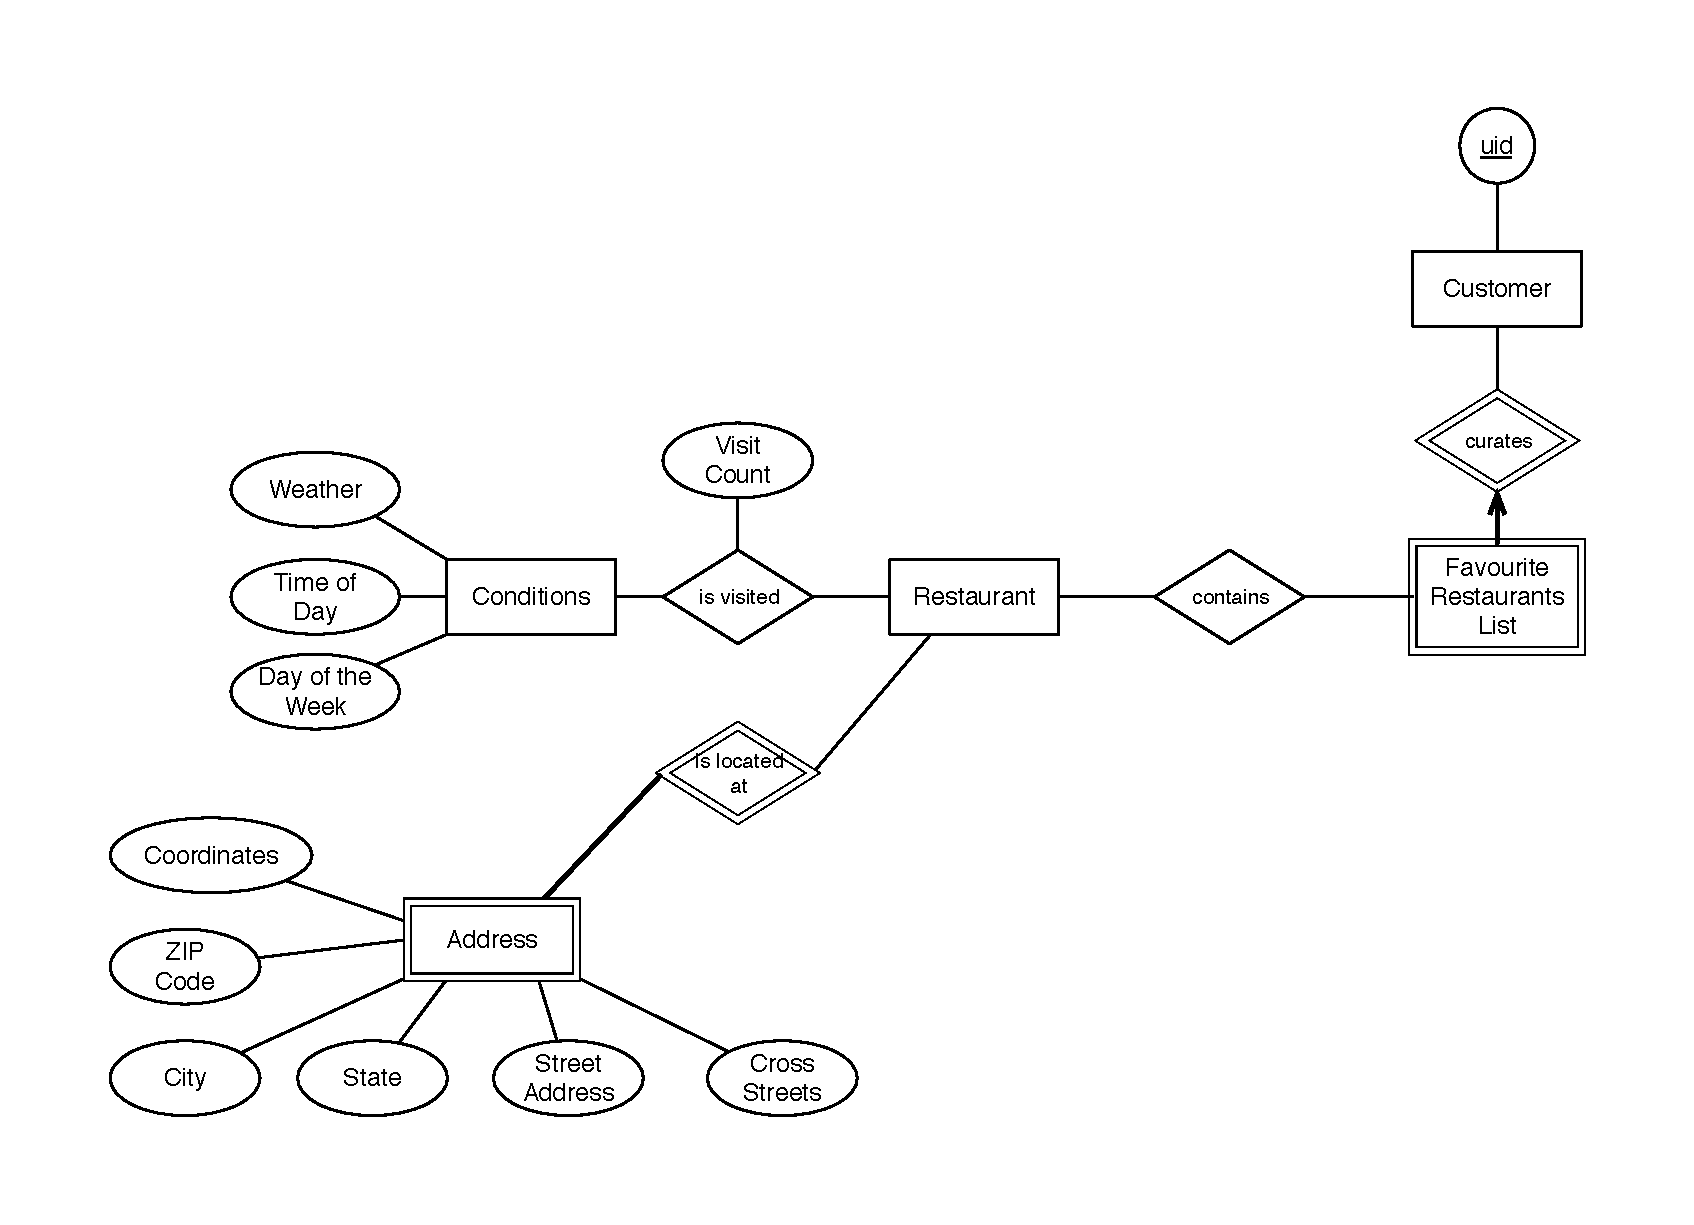
\includegraphics[angle=90,scale=0.7]{ER_diagram_simplified.pdf}

\section*{SQL Schema}

\begin{verbatim}
CREATE TABLE User(
  uid int,
  name text,
  lid int,
  PRIMARY KEY (uid)
  FOREIGN KEY (lid) REFERENCES User_Location
)

CREATE TABLE Rstrnt_of_UserLike(
  rid int,
  uid int,
  PRIMARY KEY(rid, uid)
  FOREIGN KEY (rid) REFERENCES Restaurant 
    ON DELETE CASCADE
  FOREIGN KEY (uid) REFERENCES User
    ON DELETE CASCADE
)

CREATE TABLE Restaurant(
  rid int,
  aid int NOT NULL, 
  rate int,
  PRIMARY KEY (rid)
  FOREIGN KEY (aid, rid) REFERENCES Address
    ON DELETE NO ACTION
)

CREATE TABLE Address(
  aid int,
  rid int,
  coordinate text,
  zip int,
  city text,
  state text,
  st_addr text,
  cross_st text,
  PRIMARY KEY (aid, rid)
  FOREIGN KEY (rid) REFERENCES Restaurant
    ON DELETE CASCADE
)

CREATE TABLE User_Location(
  lid int,
  uid int,
  coordinate text,
  zip int,
  city text,
  state text,
  st_addr text,
  cross_st text,
  PRIMARY KEY(lid, uid)
  FOREIGN KEY (uid) REFERENCES User
    ON DELETE CASCADE
)

CREATE TABLE Condition( -- our prebuilt table, no modifications allowed
  cid int,
  day_of_week int, -- 1~7
  weather text, -- sunny, rainy, snowy, cloudy
  time int, -- 0~24
  PRIMARY KEY (cid)
)

CREATE TABLE Visit(
  rid int,
  cid int,
  count int,
  PRIMARY KEY(rid, cid)
  FOREIGN KEY (rid) REFERENCES Restaurant
    ON DELETE CASCADE
  FOREIGN KEY (cid) REFERENCES Condition
    ON DELETE CASCADE
)
\end{verbatim}

\end{document}